
%% bare_conf.tex
%% V1.3
%% 2007/01/11
%% by Michael Shell
%% See:
%% http://www.michaelshell.org/
%% for current contact information.
%%
%% This is a skeleton file demonstrating the use of IEEEtran.cls
%% (requires IEEEtran.cls version 1.7 or later) with an IEEE conference paper.
%%
%% Support sites:
%% http://www.michaelshell.org/tex/ieeetran/
%% http://www.ctan.org/tex-archive/macros/latex/contrib/IEEEtran/
%% and
%% http://www.ieee.org/

%%*************************************************************************
%% Legal Notice:
%% This code is offered as-is without any warranty either expressed or
%% implied; without even the implied warranty of MERCHANTABILITY or
%% FITNESS FOR A PARTICULAR PURPOSE! 
%% User assumes all risk.
%% In no event shall IEEE or any contributor to this code be liable for
%% any damages or losses, including, but not limited to, incidental,
%% consequential, or any other damages, resulting from the use or misuse
%% of any information contained here.
%%
%% All comments are the opinions of their respective authors and are not
%% necessarily endorsed by the IEEE.
%%
%% This work is distributed under the LaTeX Project Public License (LPPL)
%% ( http://www.latex-project.org/ ) version 1.3, and may be freely used,
%% distributed and modified. A copy of the LPPL, version 1.3, is included
%% in the base LaTeX documentation of all distributions of LaTeX released
%% 2003/12/01 or later.
%% Retain all contribution notices and credits.
%% ** Modified files should be clearly indicated as such, including  **
%% ** renaming them and changing author support contact information. **
%%
%% File list of work: IEEEtran.cls, IEEEtran_HOWTO.pdf, bare_adv.tex,
%%                    bare_conf.tex, bare_jrnl.tex, bare_jrnl_compsoc.tex
%%*************************************************************************

% *** Authors should verify (and, if needed, correct) their LaTeX system  ***
% *** with the testflow diagnostic prior to trusting their LaTeX platform ***
% *** with production work. IEEE's font choices can trigger bugs that do  ***
% *** not appear when using other class files.                            ***
% The testflow support page is at:
% http://www.michaelshell.org/tex/testflow/



% Note that the a4paper option is mainly intended so that authors in
% countries using A4 can easily print to A4 and see how their papers will
% look in print - the typesetting of the document will not typically be
% affected with changes in paper size (but the bottom and side margins will).
% Use the testflow package mentioned above to verify correct handling of
% both paper sizes by the user's LaTeX system.
%
% Also note that the "draftcls" or "draftclsnofoot", not "draft", option
% should be used if it is desired that the figures are to be displayed in
% draft mode.
%
\documentclass[conference]{IEEEtran}
% Add the compsoc option for Computer Society conferences.
%
% If IEEEtran.cls has not been installed into the LaTeX system files,
% manually specify the path to it like:
% \documentclass[conference]{../sty/IEEEtran}

\usepackage{graphicx}
\usepackage{caption}
\usepackage{float}
\usepackage{subfig}

% Some very useful LaTeX packages include:
% (uncomment the ones you want to load)


% *** MISC UTILITY PACKAGES ***
%
%\usepackage{ifpdf}
% Heiko Oberdiek's ifpdf.sty is very useful if you need conditional
% compilation based on whether the output is pdf or dvi.
% usage:
% \ifpdf
%   % pdf code
% \else
%   % dvi code
% \fi
% The latest version of ifpdf.sty can be obtained from:
% http://www.ctan.org/tex-archive/macros/latex/contrib/oberdiek/
% Also, note that IEEEtran.cls V1.7 and later provides a builtin
% \ifCLASSINFOpdf conditional that works the same way.
% When switching from latex to pdflatex and vice-versa, the compiler may
% have to be run twice to clear warning/error messages.






% *** CITATION PACKAGES ***
%
%\usepackage{cite}
% cite.sty was written by Donald Arseneau
% V1.6 and later of IEEEtran pre-defines the format of the cite.sty package
% \cite{} output to follow that of IEEE. Loading the cite package will
% result in citation numbers being automatically sorted and properly
% "compressed/ranged". e.g., [1], [9], [2], [7], [5], [6] without using
% cite.sty will become [1], [2], [5]--[7], [9] using cite.sty. cite.sty's
% \cite will automatically add leading space, if needed. Use cite.sty's
% noadjust option (cite.sty V3.8 and later) if you want to turn this off.
% cite.sty is already installed on most LaTeX systems. Be sure and use
% version 4.0 (2003-05-27) and later if using hyperref.sty. cite.sty does
% not currently provide for hyperlinked citations.
% The latest version can be obtained at:
% http://www.ctan.org/tex-archive/macros/latex/contrib/cite/
% The documentation is contained in the cite.sty file itself.






% *** GRAPHICS RELATED PACKAGES ***
%
\ifCLASSINFOpdf
  % \usepackage[pdftex]{graphicx}
  % declare the path(s) where your graphic files are
  % \graphicspath{{../pdf/}{../jpeg/}}
  % and their extensions so you won't have to specify these with
  % every instance of \includegraphics
  % \DeclareGraphicsExtensions{.pdf,.jpeg,.png}
\else
  % or other class option (dvipsone, dvipdf, if not using dvips). graphicx
  % will default to the driver specified in the system graphics.cfg if no
  % driver is specified.
  % \usepackage[dvips]{graphicx}
  % declare the path(s) where your graphic files are
  % \graphicspath{{../eps/}}
  % and their extensions so you won't have to specify these with
  % every instance of \includegraphics
  % \DeclareGraphicsExtensions{.eps}
\fi
% graphicx was written by David Carlisle and Sebastian Rahtz. It is
% required if you want graphics, photos, etc. graphicx.sty is already
% installed on most LaTeX systems. The latest version and documentation can
% be obtained at: 
% http://www.ctan.org/tex-archive/macros/latex/required/graphics/
% Another good source of documentation is "Using Imported Graphics in
% LaTeX2e" by Keith Reckdahl which can be found as epslatex.ps or
% epslatex.pdf at: http://www.ctan.org/tex-archive/info/
%
% latex, and pdflatex in dvi mode, support graphics in encapsulated
% postscript (.eps) format. pdflatex in pdf mode supports graphics
% in .pdf, .jpeg, .png and .mps (metapost) formats. Users should ensure
% that all non-photo figures use a vector format (.eps, .pdf, .mps) and
% not a bitmapped formats (.jpeg, .png). IEEE frowns on bitmapped formats
% which can result in "jaggedy"/blurry rendering of lines and letters as
% well as large increases in file sizes.
%
% You can find documentation about the pdfTeX application at:
% http://www.tug.org/applications/pdftex





% *** MATH PACKAGES ***
%
%\usepackage[cmex10]{amsmath}
% A popular package from the American Mathematical Society that provides
% many useful and powerful commands for dealing with mathematics. If using
% it, be sure to load this package with the cmex10 option to ensure that
% only type 1 fonts will utilized at all point sizes. Without this option,
% it is possible that some math symbols, particularly those within
% footnotes, will be rendered in bitmap form which will result in a
% document that can not be IEEE Xplore compliant!
%
% Also, note that the amsmath package sets \interdisplaylinepenalty to 10000
% thus preventing page breaks from occurring within multiline equations. Use:
%\interdisplaylinepenalty=2500
% after loading amsmath to restore such page breaks as IEEEtran.cls normally
% does. amsmath.sty is already installed on most LaTeX systems. The latest
% version and documentation can be obtained at:
% http://www.ctan.org/tex-archive/macros/latex/required/amslatex/math/





% *** SPECIALIZED LIST PACKAGES ***
%
%\usepackage{algorithmic}
% algorithmic.sty was written by Peter Williams and Rogerio Brito.
% This package provides an algorithmic environment fo describing algorithms.
% You can use the algorithmic environment in-text or within a figure
% environment to provide for a floating algorithm. Do NOT use the algorithm
% floating environment provided by algorithm.sty (by the same authors) or
% algorithm2e.sty (by Christophe Fiorio) as IEEE does not use dedicated
% algorithm float types and packages that provide these will not provide
% correct IEEE style captions. The latest version and documentation of
% algorithmic.sty can be obtained at:
% http://www.ctan.org/tex-archive/macros/latex/contrib/algorithms/
% There is also a support site at:
% http://algorithms.berlios.de/index.html
% Also of interest may be the (relatively newer and more customizable)
% algorithmicx.sty package by Szasz Janos:
% http://www.ctan.org/tex-archive/macros/latex/contrib/algorithmicx/




% *** ALIGNMENT PACKAGES ***
%
%\usepackage{array}
% Frank Mittelbach's and David Carlisle's array.sty patches and improves
% the standard LaTeX2e array and tabular environments to provide better
% appearance and additional user controls. As the default LaTeX2e table
% generation code is lacking to the point of almost being broken with
% respect to the quality of the end results, all users are strongly
% advised to use an enhanced (at the very least that provided by array.sty)
% set of table tools. array.sty is already installed on most systems. The
% latest version and documentation can be obtained at:
% http://www.ctan.org/tex-archive/macros/latex/required/tools/


%\usepackage{mdwmath}
%\usepackage{mdwtab}
% Also highly recommended is Mark Wooding's extremely powerful MDW tools,
% especially mdwmath.sty and mdwtab.sty which are used to format equations
% and tables, respectively. The MDWtools set is already installed on most
% LaTeX systems. The lastest version and documentation is available at:
% http://www.ctan.org/tex-archive/macros/latex/contrib/mdwtools/


% IEEEtran contains the IEEEeqnarray family of commands that can be used to
% generate multiline equations as well as matrices, tables, etc., of high
% quality.


%\usepackage{eqparbox}
% Also of notable interest is Scott Pakin's eqparbox package for creating
% (automatically sized) equal width boxes - aka "natural width parboxes".
% Available at:
% http://www.ctan.org/tex-archive/macros/latex/contrib/eqparbox/





% *** SUBFIGURE PACKAGES ***
%\usepackage[tight,footnotesize]{subfigure}
% subfigure.sty was written by Steven Douglas Cochran. This package makes it
% easy to put subfigures in your figures. e.g., "Figure 1a and 1b". For IEEE
% work, it is a good idea to load it with the tight package option to reduce
% the amount of white space around the subfigures. subfigure.sty is already
% installed on most LaTeX systems. The latest version and documentation can
% be obtained at:
% http://www.ctan.org/tex-archive/obsolete/macros/latex/contrib/subfigure/
% subfigure.sty has been superceeded by subfig.sty.



%\usepackage[caption=false]{caption}
%\usepackage[font=footnotesize]{subfig}
% subfig.sty, also written by Steven Douglas Cochran, is the modern
% replacement for subfigure.sty. However, subfig.sty requires and
% automatically loads Axel Sommerfeldt's caption.sty which will override
% IEEEtran.cls handling of captions and this will result in nonIEEE style
% figure/table captions. To prevent this problem, be sure and preload
% caption.sty with its "caption=false" package option. This is will preserve
% IEEEtran.cls handing of captions. Version 1.3 (2005/06/28) and later 
% (recommended due to many improvements over 1.2) of subfig.sty supports
% the caption=false option directly:
%\usepackage[caption=false,font=footnotesize]{subfig}
%
% The latest version and documentation can be obtained at:
% http://www.ctan.org/tex-archive/macros/latex/contrib/subfig/
% The latest version and documentation of caption.sty can be obtained at:
% http://www.ctan.org/tex-archive/macros/latex/contrib/caption/




% *** FLOAT PACKAGES ***
%
%\usepackage{fixltx2e}
% fixltx2e, the successor to the earlier fix2col.sty, was written by
% Frank Mittelbach and David Carlisle. This package corrects a few problems
% in the LaTeX2e kernel, the most notable of which is that in current
% LaTeX2e releases, the ordering of single and double column floats is not
% guaranteed to be preserved. Thus, an unpatched LaTeX2e can allow a
% single column figure to be placed prior to an earlier double column
% figure. The latest version and documentation can be found at:
% http://www.ctan.org/tex-archive/macros/latex/base/



%\usepackage{stfloats}
% stfloats.sty was written by Sigitas Tolusis. This package gives LaTeX2e
% the ability to do double column floats at the bottom of the page as well
% as the top. (e.g., "\begin{figure*}[!b]" is not normally possible in
% LaTeX2e). It also provides a command:
%\fnbelowfloat
% to enable the placement of footnotes below bottom floats (the standard
% LaTeX2e kernel puts them above bottom floats). This is an invasive package
% which rewrites many portions of the LaTeX2e float routines. It may not work
% with other packages that modify the LaTeX2e float routines. The latest
% version and documentation can be obtained at:
% http://www.ctan.org/tex-archive/macros/latex/contrib/sttools/
% Documentation is contained in the stfloats.sty comments as well as in the
% presfull.pdf file. Do not use the stfloats baselinefloat ability as IEEE
% does not allow \baselineskip to stretch. Authors submitting work to the
% IEEE should note that IEEE rarely uses double column equations and
% that authors should try to avoid such use. Do not be tempted to use the
% cuted.sty or midfloat.sty packages (also by Sigitas Tolusis) as IEEE does
% not format its papers in such ways.





% *** PDF, URL AND HYPERLINK PACKAGES ***
%
%\usepackage{url}
% url.sty was written by Donald Arseneau. It provides better support for
% handling and breaking URLs. url.sty is already installed on most LaTeX
% systems. The latest version can be obtained at:
% http://www.ctan.org/tex-archive/macros/latex/contrib/misc/
% Read the url.sty source comments for usage information. Basically,
% \url{my_url_here}.





% *** Do not adjust lengths that control margins, column widths, etc. ***
% *** Do not use packages that alter fonts (such as pslatex).         ***
% There should be no need to do such things with IEEEtran.cls V1.6 and later.
% (Unless specifically asked to do so by the journal or conference you plan
% to submit to, of course. )


% correct bad hyphenation here
\hyphenation{op-tical net-works semi-conduc-tor}


\begin{document}
%
% paper title
% can use linebreaks \\ within to get better formatting as desired
\title{Analysis of Particle Filters as an Effective Approach to Handling Concept Drift in Streaming Data}


% author names and affiliations
% use a multiple column layout for up to three different
% affiliations
\author{\IEEEauthorblockN{Tegjyot Singh Sethi}
\IEEEauthorblockA{Computer Engineering and Computer Science Department\\
University of Louisville\\
Louisville, KY\\
Email: t0seth01@louisville.edu}
}
% conference papers do not typically use \thanks and this command
% is locked out in conference mode. If really needed, such as for
% the acknowledgment of grants, issue a \IEEEoverridecommandlockouts
% after \documentclass

% for over three affiliations, or if they all won't fit within the width
% of the page, use this alternative format:
% 
%\author{\IEEEauthorblockN{Michael Shell\IEEEauthorrefmark{1},
%Homer Simpson\IEEEauthorrefmark{2},
%James Kirk\IEEEauthorrefmark{3}, 
%Montgomery Scott\IEEEauthorrefmark{3} and
%Eldon Tyrell\IEEEauthorrefmark{4}}
%\IEEEauthorblockA{\IEEEauthorrefmark{1}School of Electrical and Computer Engineering\\
%Georgia Institute of Technology,
%Atlanta, Georgia 30332--0250\\ Email: see http://www.michaelshell.org/contact.html}
%\IEEEauthorblockA{\IEEEauthorrefmark{2}Twentieth Century Fox, Springfield, USA\\
%Email: homer@thesimpsons.com}
%\IEEEauthorblockA{\IEEEauthorrefmark{3}Starfleet Academy, San Francisco, California 96678-2391\\
%Telephone: (800) 555--1212, Fax: (888) 555--1212}
%\IEEEauthorblockA{\IEEEauthorrefmark{4}Tyrell Inc., 123 Replicant Street, Los Angeles, California 90210--4321}}




% use for special paper notices
%\IEEEspecialpapernotice{(Invited Paper)}




% make the title area
\maketitle


\begin{abstract}
%\boldmath
The abstract goes here.
\end{abstract}
% IEEEtran.cls defaults to using nonbold math in the Abstract.
% This preserves the distinction between vectors and scalars. However,
% if the conference you are submitting to favors bold math in the abstract,
% then you can use LaTeX's standard command \boldmath at the very start
% of the abstract to achieve this. Many IEEE journals/conferences frown on
% math in the abstract anyway.

% no keywords




% For peer review papers, you can put extra information on the cover
% page as needed:
% \ifCLASSOPTIONpeerreview
% \begin{center} \bfseries EDICS Category: 3-BBND \end{center}
% \fi
%
% For peerreview papers, this IEEEtran command inserts a page break and
% creates the second title. It will be ignored for other modes.
\IEEEpeerreviewmaketitle
% An example of a floating figure using the graphicx package.
% Note that \label must occur AFTER (or within) \caption.
% For figures, \caption should occur after the \includegraphics.
% Note that IEEEtran v1.7 and later has special internal code that
% is designed to preserve the operation of \label within \caption
% even when the captionsoff option is in effect. However, because
% of issues like this, it may be the safest practice to put all your
% \label just after \caption rather than within \caption{}.
%
% Reminder: the "draftcls" or "draftclsnofoot", not "draft", class
% option should be used if it is desired that the figures are to be
% displayed while in draft mode.
%
%\begin{figure}[!t]
%\centering
%\includegraphics[width=2.5in]{myfigure}
% where an .eps filename suffix will be assumed under latex, 
% and a .pdf suffix will be assumed for pdflatex; or what has been declared
% via \DeclareGraphicsExtensions.
%\caption{Simulation Results}
%\label{fig_sim}
%\end{figure}

% Note that IEEE typically puts floats only at the top, even when this
% results in a large percentage of a column being occupied by floats.


% An example of a double column floating figure using two subfigures.
% (The subfig.sty package must be loaded for this to work.)
% The subfigure \label commands are set within each subfloat command, the
% \label for the overall figure must come after \caption.
% \hfil must be used as a separator to get equal spacing.
% The subfigure.sty package works much the same way, except \subfigure is
% used instead of \subfloat.
%
%\begin{figure*}[!t]
%\centerline{\subfloat[Case I]\includegraphics[width=2.5in]{subfigcase1}%
%\label{fig_first_case}}
%\hfil
%\subfloat[Case II]{\includegraphics[width=2.5in]{subfigcase2}%
%\label{fig_second_case}}}
%\caption{Simulation results}
%\label{fig_sim}
%\end{figure*}
%
% Note that often IEEE papers with subfigures do not employ subfigure
% captions (using the optional argument to \subfloat), but instead will
% reference/describe all of them (a), (b), etc., within the main caption.


% An example of a floating table. Note that, for IEEE style tables, the 
% \caption command should come BEFORE the table. Table text will default to
% \footnotesize as IEEE normally uses this smaller font for tables.
% The \label must come after \caption as always.
%
%\begin{table}[!t]
%% increase table row spacing, adjust to taste
%\renewcommand{\arraystretch}{1.3}
% if using array.sty, it might be a good idea to tweak the value of
% \extrarowheight as needed to properly center the text within the cells
%\caption{An Example of a Table}
%\label{table_example}
%\centering
%% Some packages, such as MDW tools, offer better commands for making tables
%% than the plain LaTeX2e tabular which is used here.
%\begin{tabular}{|c||c|}
%\hline
%One & Two\\
%\hline
%Three & Four\\
%\hline
%\end{tabular}
%\end{table}


% Note that IEEE does not put floats in the very first column - or typically
% anywhere on the first page for that matter. Also, in-text middle ("here")
% positioning is not used. Most IEEE journals/conferences use top floats
% exclusively. Note that, LaTeX2e, unlike IEEE journals/conferences, places
% footnotes above bottom floats. This can be corrected via the \fnbelowfloat
% command of the stfloats package.

\section{Introduction}
With the Big Data revolution, there is an ever increasing influx  of data which is diverse, dynamic and distributed. The view of data is shifting from one that assumes that data is available in large databases ready for analysis, to one where the data is viewed as a dynamic stream which evolves over time and predictions need to be made in time for them to be of any value. Analyzing streaming data poses unique challenges in terms of making efficient use of time and memory resources and being able to provide good predictive capabilities all at the same time. An additional challenge to mining streaming data is that the models need to adapt to changes to the environment, known as Concept Drift\cite{Tsymbal(2004)}\cite{Zliobaite(2009)}. Concept drift makes any model obsolete unless it is retrained on a part of the stream to account for the changes in the input data distribution.

In this paper, a particle filtering based approach to mining data streams, as proposed in \cite{pflr}, is analyzed. Particle filtering is a sequential Monte Carlo approach capable of estimating the posterior distribution of a system's state over time. Particle filters have been used in literature for object tracking applications \cite{Ristic}. With modifications to the basic particle filtering algorithm to use the training accuracy as a measure of particle's performance, instead of likelihood, the PF\_LR approach of \cite{pflr} is made amenable to be used as a stream classification system. The PF\_LR algorithm builds a classifier by combining features of all the particles, which themselves represent individual models, making it essentially an ensemble classification approach. 

The paper is organized as follows: Section 2 presents a brief overview of popular ensemble techniques used for stream classification and also presents the AUE\_NB and the LB\_HT methodologies which are used later for comparative analysis. Section 3 describes the PF\_LR approach as is used for the classification of streaming data. Section 4 presents description of datasets used and the experimental results obtained. The TJSS dataset was generated specifically for the purpose of analyzing the response of the algorithm  in different scenarios.Section 5 presents concluding remarks and avenues for further research in this area. 




\section{Literature Review}
One the most widely used techniques for dealing with streaming data classification in the presence of concept drift is the use of ensemble of classifiers \cite{Kong and Yu(2011)}. The effectiveness of ensemble classifiers stems from combining the predictions of several weak classifiers to produce an overall strong prediction. Traditional ensemble classifiers for streams, such as the Simple Voting Ensemble (SVE) \cite{Street and Kim(2001)} and the Weighted Ensemble(WE) \cite{Wang 2003}\cite{Littlestone and Warmuth(1989)}, employ a window based chunk approach. The SVE builds an ensemble using all samples within a chunk and then aggregates the predictions based on a majority vote. The WE also make classifiers on each chunk, but uses a weighted aggregation with higher weight given to models that perform well on the most recent chunk. Dynamic ensembles which can grow and prune models when needed are described in \cite{Kolter and Maloof(2007)}, and are more efficient as they generate classifiers only when needed.

The SEA ensemble learning methodology \cite{Street and Kim(2001)} is based on the SVE approach, while the Accuracy Updated Ensemble(AUE) and the Leverage Bagging(LB) are methodologies based on the weighted ensemble approach. In this paper, comparisons is made with the AUE approach with a Naive Bayes base classifier (AUE\_NB) and the LB with a Hoeffding tree base classifier(LB\_HT). Hoeffding trees are incremental, anytime decision tree induction algorithms that are capable of learning from massive data streams, assuming that the distribution generating examples does not change over time \cite{Hoeglinger}. Hoeffding trees exploit the fact that a small sample can often be enough to choose an optimal splitting attribute. These methodologies used for comparison are already implemented in the MOA framework from Weka \cite{moa}, and are used as is. 


\section{Particle Filtering for Classification }

\begin{figure*}
\captionsetup{justification=centering}
\centering
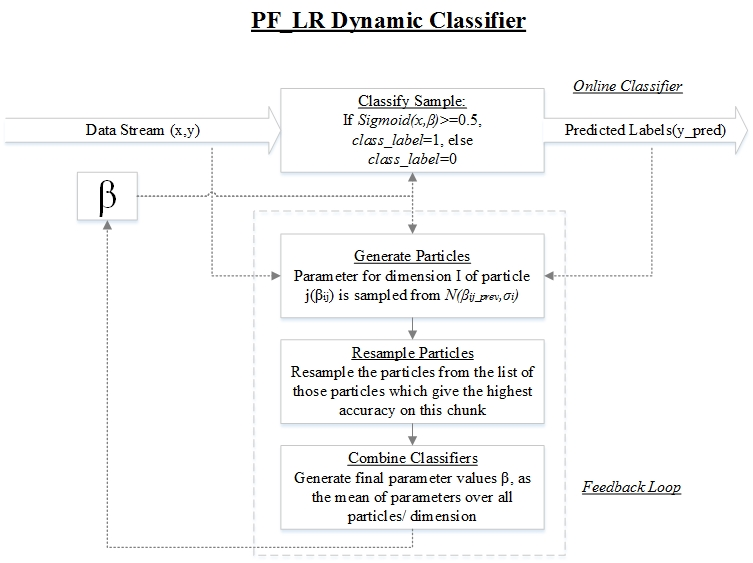
\includegraphics[scale=0.62]{fig/methodology.jpg}
\caption{Overview of PF\_LR }
\label{fig:blkoverall} 
\end{figure*}

Particle filtering is an online Monte Carlo method for performing inference in state-space models where the system evolves dynamically over time \cite{Andrieu}. It is used to estimate the posterior density of the state space by directly implementing the Bayesian inference recursion equation. Sequential importance sampling is used to approximate the likelihood function using a tractable chosen distribution. By doing this, particles in subsequent chunks are generate near the ones with high likelihood values. The basic steps in estimating the parameter $\beta$ of the system is as follows:

\begin{enumerate}
 \item  Generate M particle from the chosen proposal function $q(.|B^{n-1})$ where n is the current chunk. 
 \item Calculate M incremental weights $w_{i}^{(n|n-1)}$ for each particle, wehre the weight $w^{(n|n-1|)}$ is given as:\\
 $w^{(n|n-1|)}= \frac{p_n (\beta^n | x^n , \beta^{(n-1)})}{q_n(\beta^n|\beta^(n-1))}$ 
 Here $p(\beta,x)$ represents the posterior distribution of the model parameters and $q_n$ is the chose proposal function.
 \item Calculate the weights $w_{i}^{(1:n)} = w_{i}^{(1:n-1)} . w_{i}^{(n|n-1)}$
 \item Resample ${w_{i}^{n} , X_{i}^{1:n} }$ to find M equal weight particles ${1/N, \bar{X_i ^{1:n}}}$ 
\end{enumerate}

In the proposed methodology of \cite{pflr}(PF\_LR), a modification to the basic particle filtering approach was suggested, where instead of using the likelihood function, the training accuracy was used to generate particles in subsequent time intervals. For the task of classification the parameter $\beta$ should represent the model boundaries as such the Particle filtering algorithm will be an ensemble classification methodology with the final model boundary being a combination of the parameters of all the particles which perform well on the training set. In case of the PF\_LR, the basic model is a logistic regression model and hence $\beta$ represent the coefficient of the regression equation fit on the training data chunk. 


The description of the model's functioning is shown in Fig.~{fig:blkoverall}. Each particle in the algorithm represents a parameter set for a logistic regression model.  The \textit{Online Classifier} takes the input sample and the parameter values from the last chunk and predicts the class labels for the sample. The predicted label and the actual labels are then passed to the \textit{Feedback Loop}, where the model is retrained to maintain accuracy after a concept drift occurs. The retraining process starts with generation of particles sampled from a Normal distribution centered around the particles position form the previous chunk. The accuracy of each such particle is computed and then a Resampling step is applied to generate M particles from the set of those particles which give the highest training accuracy. This step ensures diversity in the particle set and prevents it from degenerating and getting stuck in a local optima. Since, the batch size is less than M, there are more than one particles which give  the maximum accuracy , in most chunks. The final model is generated by taking a mean of the parameters of the resampled particles. In this way the PF\_LR algorithm is similar to a bagged ensemble classifier with majority voting. The generated parameter $\beta$ are used towards the predictions in the next chunk and the cycle is repeated. The complexity of this approach is linear with \textit{O(MN)}, where M is the number of particles and N is the length of the stream. 

\section{Experimental Analysis}
In this section, the experimental evaluation is presented considering two synthetic streams and one real world streaming dataset. The performance of the analyzed PF\_LR approach is presented and compared to that of existing drift handling systems namely: the Accuracy Updated Ensemble and the Leveraged Bagging-Hoeffding Trees approach. The details of the datasets used, experimentation performed and results obtained is presented here.

\subsection{Description of Datasets used}
Two synthetic data streams: SEA \cite{Street and Kim(2001)} and TJSS stream and one real world data stream: the EM dataset\cite{Harries and Wales (1999)}\cite{Gong-De etal(2012)}, are used for performing the experimental evaluation. The datasets are described here. All attributes are normalized to the range of [0,1] using the min-max normalization approach.

\subsubsection{SEA Dataset}
The SEA dataset is a synthetic data stream of 60,000 examples, 3 attributes and 2 classes. Attributes are numeric between 0 and 10, only two are relevant. Drift occurs every 15,000 samples. The drift is generated according to the following rule: the class label is 1 for $relevant\_feature1+relevant\_feature2 < \theta_{drift}$, where $\theta_{drift}$ is a threshold which is varied as-{8,9,7,9.5}. The data stream has 10\% noise. 

\subsubsection{Synthetic TJSS Stream }
\label{sec:syntheticstream}

The TJSS stream is a synthetic two dimensional dataset which exhibits various types of dynamic drifting scenarios that can cause a model to degrade. The stream consists of 25660 samples with two classes.Some salient features of the stream are: Non spherical clusters, clusters with extensions, clusters with total reversal of class distribution, new clusters appearing over time, etc. The Fig.~\ref{fig:syntheticstream} shows the progression of the stream at incremental timestamps. In Fig.~\ref{fig:stream_1}) , the initial 10\% of the stream is shown, following which the extension of the cluster is shown in b) along with appearance of a new cluster. In c) merging clusters are demonstrated and in d, e), further extension, cluster inceptions and model drifts are exhibited by the stream. The final phase of the stream demonstrates a pure model drift where the class definition of a cluster is totally reversed keeping the model boundary undisturbed. This synthetic stream was generated to evaluate the performance of the GC3 Framework in various drifting scenarios and observe its behavior and response to each of these changes.

\begin{figure*}
\captionsetup{justification=centering}
\centering

\begin{center}
    \subfloat[10\% of TJSS stream (t=2566)]{\label{fig:stream_1}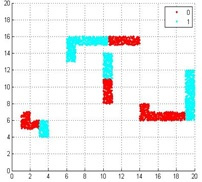
\includegraphics[scale=0.8]{fig/stream_1.jpg}}
    \subfloat[Extension of Cluster, New cluster inception (t=16840)]{\label{fig:stream_2}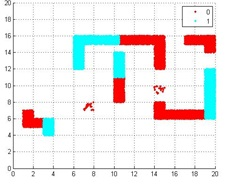
\includegraphics[scale=0.8]{fig/stream_2.jpg}}
    \subfloat[Merger of Cluster(t=17640)]{\label{fig:stream_3}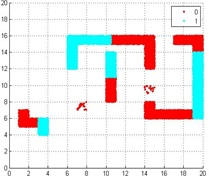
\includegraphics[scale=0.8]{fig/stream_3.jpg}}\\
     \subfloat[Extension of cluster with model shift(t=20040)]{\label{fig:stream_4}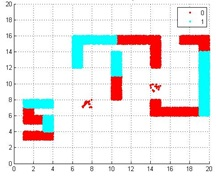
\includegraphics[scale=0.8]{fig/stream_4.jpg}}
      \subfloat[Inception of new cluster(t=23240)]{\label{fig:stream_5}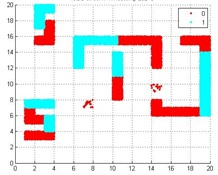
\includegraphics[scale=0.8]{fig/stream_5.jpg}}
       \subfloat[class distribution reversal(t=25660)]{\label{fig:stream_6}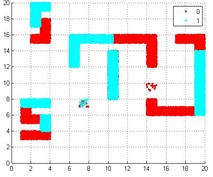
\includegraphics[scale=0.8]{fig/stream_6.jpg}}
  \end{center}
  \caption{Evolution of TJSS stream over time}
\label{fig:syntheticstream} 
\end{figure*}

\subsubsection{Electricity Market dataset}
The EM dataset were obtained from TransGrid, the electricity supplier in New South Wales, Australia. The data represents fluctuations in the electricity pricing (up/down) from May 1996 to December 1998, with the output recorded relative to a moving average of the last 24 hours. These prices were affected by various external factors such as market demand, weather and time of day; they evolve seasonally and show sensitivity only to short-term events. This data is representative of a real world scenario where the type of drift is not known in advance, is usually erratic and affected by several external factors. It enables us to gain insight into the performance of the framework in a real world scenarios where no prior information on the type of concept drift can be known. The dataset here considers only the last 5 attributes as relevant, contains 45312 samples and two classes. 

\subsection{Parameters and Methodologies used}
The classification performance of the PF\_LR methodology is compared against the Accuracy Updated Ensemble and the Leverage Bagging Hoeffding Tree approach, which are available in the MOA tool of Weka \cite{moa}. The PF\_LR approach was implemented in Python and the performance of all results were compared based on the accuracy of classification. The accuracy is also evaluated against a traditional static baseline Logistic Regression model trained on 10\% of the stream, to assess the efficacy of the models as a drift handling system and also to establish the datasets to be suitable for such a kind of evaluation. 

The PF\_LR methodology was evaluated on 50 for the two synthetic streams and 10 samples/chunk for the EM stream. The $\sigma_i$ was taken as 0.1 for all i as specified in \cite{pflr}. The number of particles was taken as 100. The LB\_HT approach and the AUE\_NB were used with all default parameters in Weka and the accuracy was evaluated with the the same chunk size as used for the PF\_LR approach. The accuracy was reported 1000 samples at a time to see the performance over time. 

\subsection{Results and Analysis}
The four models are compared over the streams and the average accuracy over time is presented in Fig.~\ref{fig:runningaccuracy}. The accuracy over time/chunk is given in Fig.~\ref{fig:chunkaccuracy}, where the average accuracy over 1000 samples is presented for a more fine grained assessment of the drift handling mechanism of the methodologies. The comparison of accuracy is presented in Fig.~\ref{fig:overallaccuracy} and Table.~\ref{table:comparison}. The PF\_LR was run 10 times for each data stream and the mean accuracy values is presented.

The red line in Fig.~\ref{fig:runningaccuracy} shows the baseline which is the performance of a static model trained on 10\% of the initial stream. The average accuracy of the LB\_HT, AUE\_NB and the PF\_LR models all have better performance than the traditional model. This indicates that the drifts all have significant dynamics over time and the three drift handling  methodologies are capable of detecting and managing changes in the stream. The LB\_HT and the PF\_LR models perform well over the three datasets. 


\begin{figure*}
\captionsetup{justification=centering}
\centering
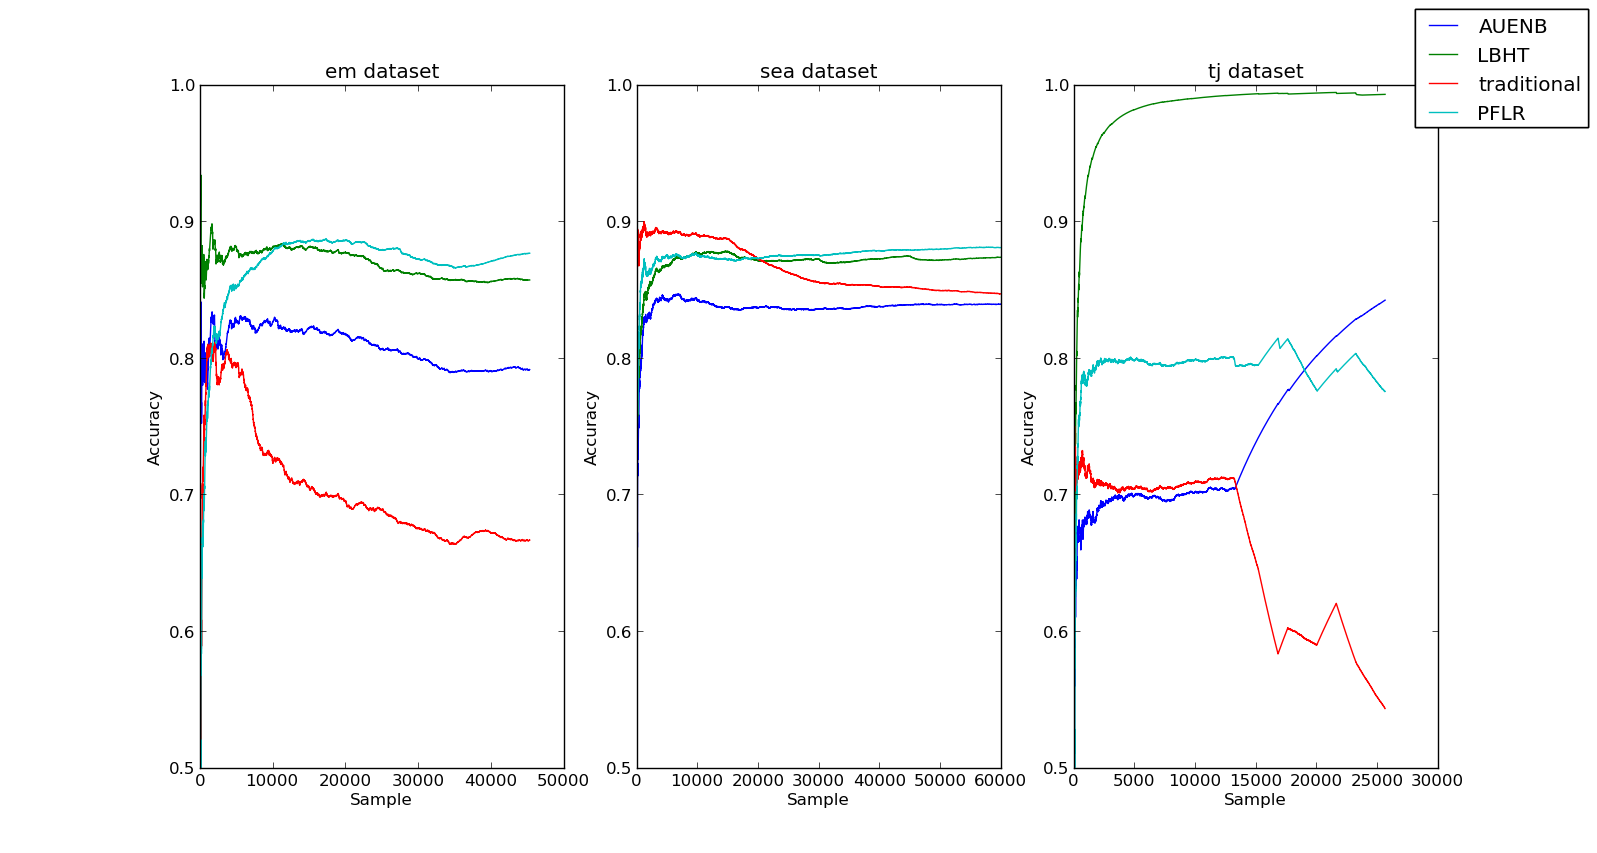
\includegraphics[scale=0.4]{fig/running_accuracy.png}
\caption{Accuracy comparison over time}
\label{fig:runningaccuracy} 
\end{figure*}

\begin{figure}
\captionsetup{justification=centering}
\centering
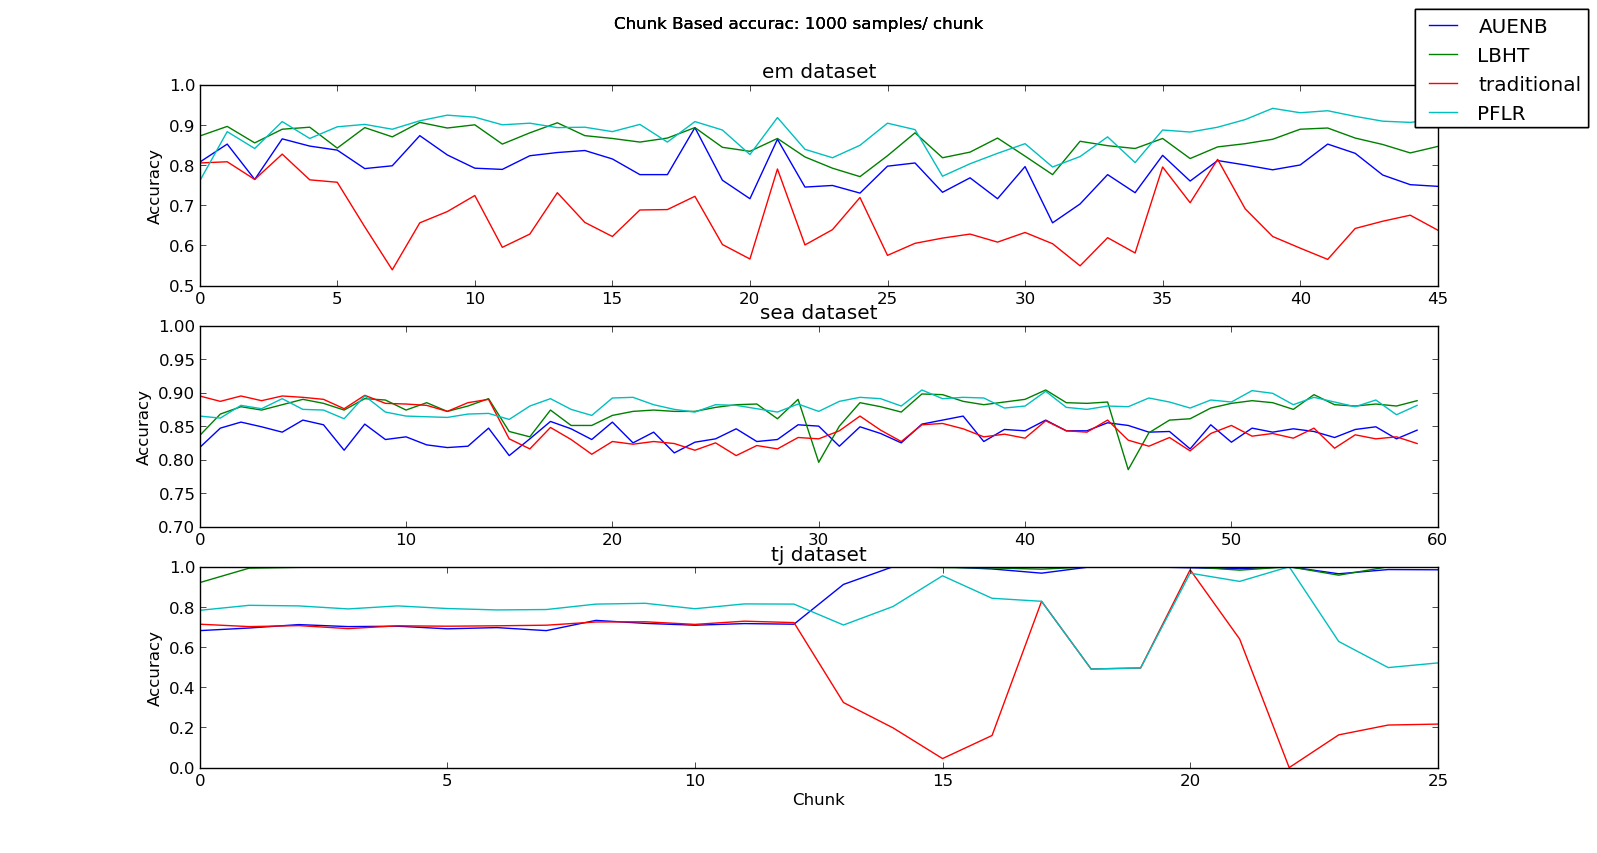
\includegraphics[scale=0.2]{fig/chunk_accuracy.png}
\caption{Accuracy comparison over time 1000 samples/chunk}
\label{fig:chunkaccuracy} 
\end{figure}

The chunk accuracy plots of Fig.~\ref{fig:chunkaccuracy} demonstrate the behaviour of the PF\_LR model under different drifting scenarios. For the SEA data stream, the drift occurs at chunk 15,30,45,60. This can be seen as a dip at these chunk values and then a subsequent rise indicative of the drift  being handled effectively. For the traditional model, each drift leads to a continuous loss in performance from  which the system has no way of recovering. In case of the TJSS stream, there is no drift till chunk 13, this is indicated by the accuracies of all models following a similar trajectories. Following the chunk 13, there are different drifting aspect of the stream which are effectively handled by the PF\_LR to give better performance than the the traditional static model. However, it can be seen that the AUE\_NB and the LB\_HT perform much better on this data stream. The EM stream has unknown drifting components and as such is most representative of a real world scenario. The PF\_LR performs well on this data demonstrating its ability to be used effectively in scenarios where the drift is unknown and unpredictable. The overall accuracy at the end of the stream is presented in Table.~\ref{table:comparison}.


\begin{table}
\centering
\caption{Accuracy comparison of LB\_HT,AUE\_NB,PF\_LR and the traditional model}
\begin{tabular}{l l l l} % centered columns (4 columns) 
\hline\noalign{\smallskip}
Model/DataStream & SEA & TJSS & EM\\
\noalign{\smallskip}\hline\noalign{\smallskip}
Pf\_LR &0.8792$\pm$0.004 &0.7095$\pm$0.003 & 0.849$\pm$0.002\\
Traditional &0.8467 &0.5432&0.6665  \\
LB\_HT &0.8735& 0.9928 &0.8569  \\
AUE\_NB &0.8392 &0.8422 &0.7913  \\ 
\noalign{\smallskip}\hline
\end{tabular} 
\label{table:comparison}
\end{table}

\begin{figure}
\captionsetup{justification=centering}
\centering
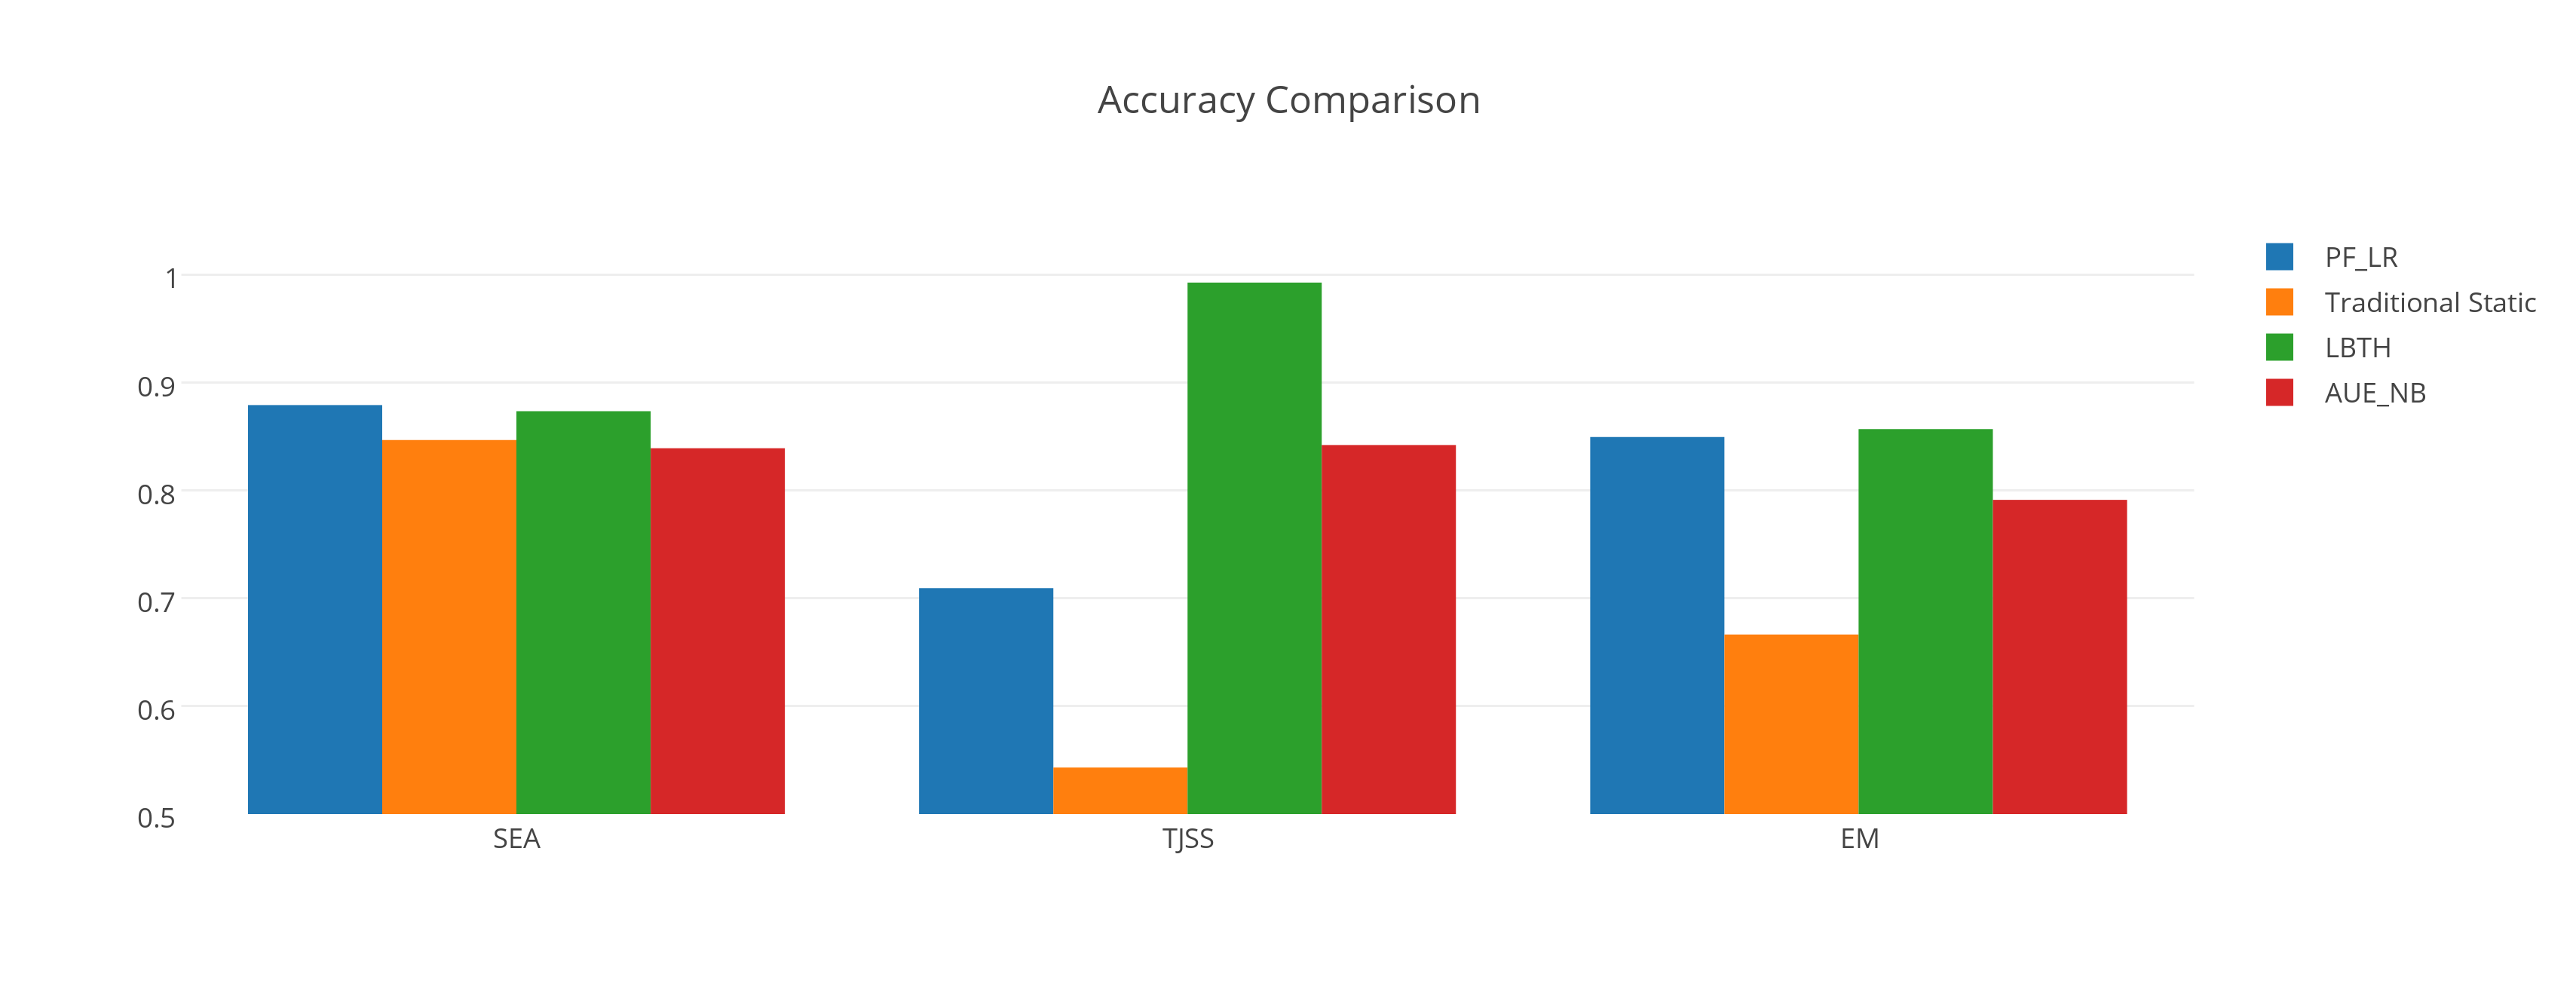
\includegraphics[scale=0.3]{fig/accuracy_comparison.png}
\caption{Overall performance comparison}
\label{fig:overallaccuracy} 
\end{figure}

\subsubsection{Discussion}
The PF\_LR methodology performs better than the traditional static model and produces comparative results when compared to other drift handling methodologies. However, in case of the TJSS stream, its performance is not as good. The TJSS stream was generated to analyze the performance of a drift handling system in its ability to handle various types of drifts. An analysis of the predicted stream accuracy per chunk of 100 samples provides for a fine grained understanding of the performance of the PF\_LR algorithm, as depicted in Fig.~\ref{fig:chunk_100_tr}. From the figure it can be seen that the model is able to recognize most types of drifts and is able to recover from them fairly soon. This is indicated by a dip in the accuracy followed by a quick ascent. 

\begin{figure}
\captionsetup{justification=centering}
\centering
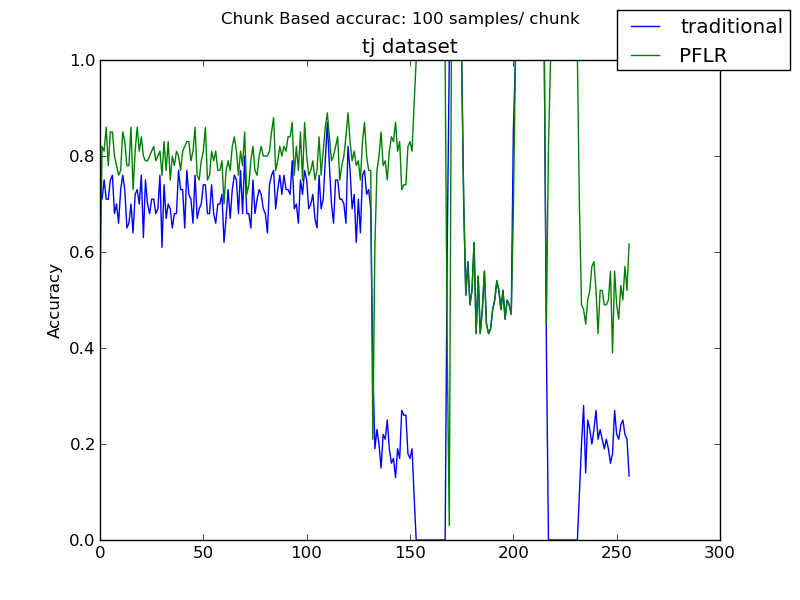
\includegraphics[scale=0.4]{fig/chunk_100_traditional_PFLR.png}
\caption{Accuracy per chunk of 100 samples for the traditional and PF\_LR model}
\label{fig:chunk_100_tr} 
\end{figure}


From the Fig.~\ref{fig:chunk_100_tr} it can be seen that the PF\_LR algorithm follows similar trajectory as the traditional static model till the chunk 130. This is the portion of the stream which does not demonstrate any drift. After this chunk, the performance of the PF\_LR sample is increases indicating its ability to adapt well to changes in data distribution (Changes in the T portion of the dataset) that maintain the class boundary. From chunk 180-210, it is seen that the performance of both models is similar. This is the portion of the stream which has extension in a direction opposite to the established class boundary. The PF\_LR model has a hard time recognizing these changes. It is however able to account for the newly formed S cluster as seen in Fig.~\ref{fig:syntheticstream} e). The final change in the stream which represents a reversal of class labels while maintaining the boundary, causes a loss in the PF\_LR's performance. But as can be seen from the Fig.~\ref{fig:chunk_100_tr}, this drop in performance is not as bad as the traditional model, implying the ability of the particle filtering model to react effectively although slowly to the drift purely in the class distribution. 

\begin{figure}
\captionsetup{justification=centering}
\centering
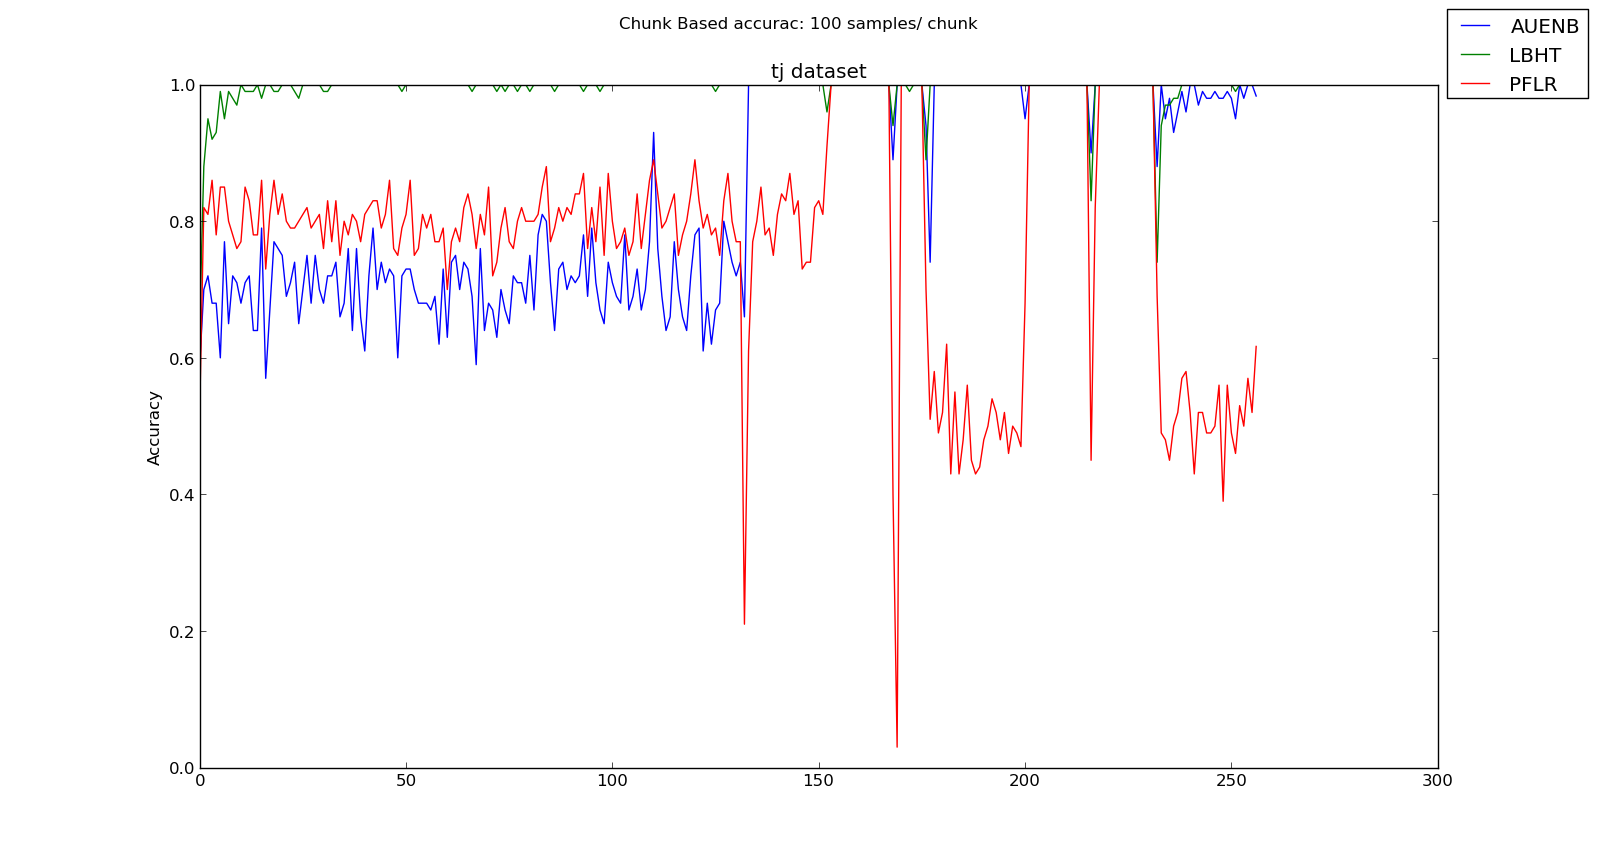
\includegraphics[scale=0.22]{fig/chunk_100_drifthandlers.png}
\caption{Accuracy per chunk of 100 samples}
\label{fig:chunk_dh_100} 
\end{figure}

The Fig.~\ref{fig:chunk_dh_100}, compares the performance of the drift handling methodologies on the TJSS stream. It can be seen that the LB\_HT performs exceptionally well on this dataset. This is indicative of its predictive power over non noisy data streams, irrespective of the nature and frequency of drifts. the AUE\_NB approach also performs well on the stream. However, the initial performance before the drift is lower than any of the other methodologies. It should be observed that all the methodologies have similar width of recovery, in case the drift is detected by them. The PF\_LR and the AUE\_NB have higher drop in accruacy but all of them recover by the same chunk size to give higher prediction accuracy. A comparison of these algorithms indicate that the LB\_HT and the AUE\_NB are superior than PF\_LR in detecting local drifts where a portion of the input data distribution might change while keeping the rest constant. The PF\_LR is effective in capturing drifts over noisy real world streams (like the EM stream), especially in scenarios where the drift effects the entire input data distribution globally. 


\section{Conclusion and Future work}
In this paper a particle filtering based online classification approach, the PF\_LR algorithm, was analyzed as a viable candidate for handling concept drift in streaming data. The algorithm was analyzed on two synthetic datasets, SEA and TJSS stream, and one real world dataset, the EM stream. The results obtained showed that the PF\_LR algorithm is an effective drift handling system as it always performs better than a static model trained on only a subset of the stream. When compared with other state of the art drift handling systems, the AUE\_NB and the LB\_HT,it's performance was competitive. The PF\_LR was able to handle all types of drifts but had a hard time in detecting drifts which affect a subset of the data space, at a time. However, its ability to perform drift handling without explicit drift detection, its linear complexity and its robustness to noise makes it attractive for use as a stream classification system. 

This paper assumed that all input samples are labeled and that the label is available immediately after a chunk is processed. This is not true in a streaming environment milieu as labeling can be both time consuming and costly. Thus, the efficacy of using the PF\_LR methodology with only partial labeling is an interesting area fro further research. 


% trigger a \newpage just before the given reference
% number - used to balance the columns on the last page
% adjust value as needed - may need to be readjusted if
% the document is modified later
%\IEEEtriggeratref{8}
% The "triggered" command can be changed if desired:
%\IEEEtriggercmd{\enlargethispage{-5in}}

% references section

% can use a bibliography generated by BibTeX as a .bbl file
% BibTeX documentation can be easily obtained at:
% http://www.ctan.org/tex-archive/biblio/bibtex/contrib/doc/
% The IEEEtran BibTeX style support page is at:
% http://www.michaelshell.org/tex/ieeetran/bibtex/
%\bibliographystyle{IEEEtran}
% argument is your BibTeX string definitions and bibliography database(s)
%\bibliography{IEEEabrv,../bib/paper}
%
% <OR> manually copy in the resultant .bbl file
% set second argument of \begin to the number of references
% (used to reserve space for the reference number labels box)
\begin{thebibliography}{16}

\bibitem{Ristic}
Ristic B, Arulampalam S, Gordon N (2004) Beyond the Kalman filter: Particle filters for tracking applications. Artech house.

\bibitem{Andrieu}
Andrieu C, Doucet A, Holenstein R (2010). Particle markov chain monte carlo methods. Journal of the Royal Statistical Society: Series B (Statistical Methodology), 72(3), 269-342.

 \bibitem{Zliobaite(2009)}
Zliobaite I (2009) Learning under concept drift: an overview. Tech. rep.,
  Technical report, Vilnius University, 2009 techniques, related areas,
  applications Subjects: Artificial Intelligence

\bibitem{Tsymbal(2004)}
Tsymbal A (2004) The problem of concept drift: definitions and related work.
  Computer Science Department, Trinity College Dublin

\bibitem{Street and Kim(2001)}
Street WN, Kim Y (2001) A streaming ensemble algorithm {(SEA)} for large-scale
  classification. In: Proceedings of the seventh ACM SIGKDD international
  conference on Knowledge discovery and data mining, ACM, pp 377--382

\bibitem{Littlestone and Warmuth(1989)}
Littlestone N, Warmuth MK (1989) The weighted majority algorithm. In: 30th
  Annual Symposium on Foundations of Computer Science, IEEE, pp 256--261

\bibitem{Kolter and Maloof(2007)}
Kolter JZ, Maloof MA (2007) Dynamic weighted majority: An ensemble method for
  drifting concepts. The Journal of Machine Learning Research 8:2755--2790

\bibitem{Kong and Yu(2011)}
Kong X, Yu P (2011) An ensemble-based approach to fast classification of
  multi-label data streams. In: 7th International Conference on Collaborative
  Computing: Networking, Applications and Worksharing, IEEE, pp 95--104
  
\bibitem{Gong-De etal(2012)}
Gong-De G, Nan L, Li-Fei C (2012) Classification for concept-drifting data
  streams with limited amount of labeled data. In: International Conference on
  Automatic Control and Artificial Intelligence (ACAI 2012), IET, pp 638--644

\bibitem{Harries and Wales(1999)}
Harries M, Wales NS (1999) Splice-2 comparative evaluation: Electricity pricing

\bibitem{Rokach(2010)}
Rokach L (2010) Ensemble-based classifiers. Artificial Intelligence Review
  33(1-2):1--39

\bibitem{Chen and He(2011)}
Chen S, He H (2011) Towards incremental learning of nonstationary imbalanced
  data stream: a multiple selectively recursive approach. Evolving Systems
  2(1):35--50
  
\bibitem{Wang 2003}
Wang H, Fan W, Yu PS, Han J (2003) Mining concept-drifting data streams using
  ensemble classifiers. In: Proceedings of the ninth ACM SIGKDD international
  conference on Knowledge discovery and data mining, ACM, pp 226--235

 \bibitem{Hoeglinger}
Hoeglinger S, Pears R (2007) Use of hoeffding trees in concept based data stream mining. In: Third international conference on information and automation for sustainability ICIAFS 2007, IEEE.
  
 \bibitem{moa}
 Bifet A, et al.(2010) Moa: Massive online analysis; The Journal of Machine Learning Research 11: 1601-1604
 
 \bibitem{pflr}
 Fok R, An A, Wang X (2013) Mining Evolving Data Streams with Particle Filters.
\end{thebibliography}




% that's all folks
\end{document}


